\chapter{3D Discrete Global Grid Systems} \label{chap:3ddggs}
In the previous chapter, we reviewed the DGGS as a tool for integrating multiple geospatial datasets at varying resolutions.
However, a conventional DGGS has no inbuilt mechanism for handling the altitude(s) of geospatial data.
Instead, an extension of the data structure to the third dimension---the 3D DGGS---is needed to accommodate such 3D data natively.
This chapter argues for the need for 3D DGGS's in certain applications by exploring the downsides of a typical data flattening approach used to integrate 3D data with a 2D DGGS.
We then compare the two most common approaches used for creating a 3D DGGS: embedding and Earth-centric.
We argue for the Earth-centric approach, proposing semiregular degenerate refinement---the primary tool used in the remainder of this thesis---as a strategy to lessen the disadvantages of this type of grid.


\section{Data Flattening} \label{chap:3:flatten}
A DGGS provides a multiresolution partitioning of the Earth's surface, but no partitioning in the radial dimension.
Therefore, any geospatial data with associate altitude must be flattened to the surface for integration with a DGGS, with the original altitude stored as an attribute of the data.
In applications where data \textit{does not} need to be filtered by altitude, and altitude is used no differently than any other attribute, this is an acceptable approach.
However, if data \textit{does} need to be accessed or otherwise distinguished by altitude, then this approach is problematic.
In this case, all data of a cell must be queried and searched to find those with the required altitude(s).
Furthermore, the lack of a hierarchy in the radial dimension means data at different radial resolutions must be integrated manually as opposed to using the structure of the DGGS itself to aid in this task.
Generally speaking, any benefits gained by using a DGGS are lost in the radial dimension; this is problematic for any application that uses the radial dimension as frequently as surface ones.
For example, with aircraft collision detection and avoidance, the altitude of aircraft is just as important as their geographic coordinates.
Instead of managing altitude separately, we need an extension of the 2D DGGS that hierarchically partitions altitude in addition to the surface of the Earth.
We call this a 3D DGGS.


\section{Embedded Grids} \label{chap:3:embedded}
Treating the Earth as a fully 3D entity, it seems natural to use a conventional Euclidean space partitioning data structure such as a voxel grid or octree to manage geospatial data.
We refer to this approach as an embedding one, creating an embedded 3D DGGS.
While an embedding approach is straightforward and leverages existing data structures and algorithms, it disregards the actual shape of the Earth.
Regardless of how finely refined cells are, they can only approximate the underlying representation of the Earth: a sphere or ellipsoid (\cref{fig:embedded}).
Furthermore, cells do not align with the Earth's surface, which means cells have no consistent orientation of what direction represents an increasing or decreasing altitude (up and down).
Because of this, traversing along the surface of the Earth (or any other constant altitude) becomes a non-straightforward operation that requires a ``zig-zagging'' path.
An example application where this is problematic goes here.
Due to the multi-sphere structure of the Earth, these challenges also manifest when dealing with different subterranean and atmospheric layers.


\begin{figure}[ht!]
	\centering
	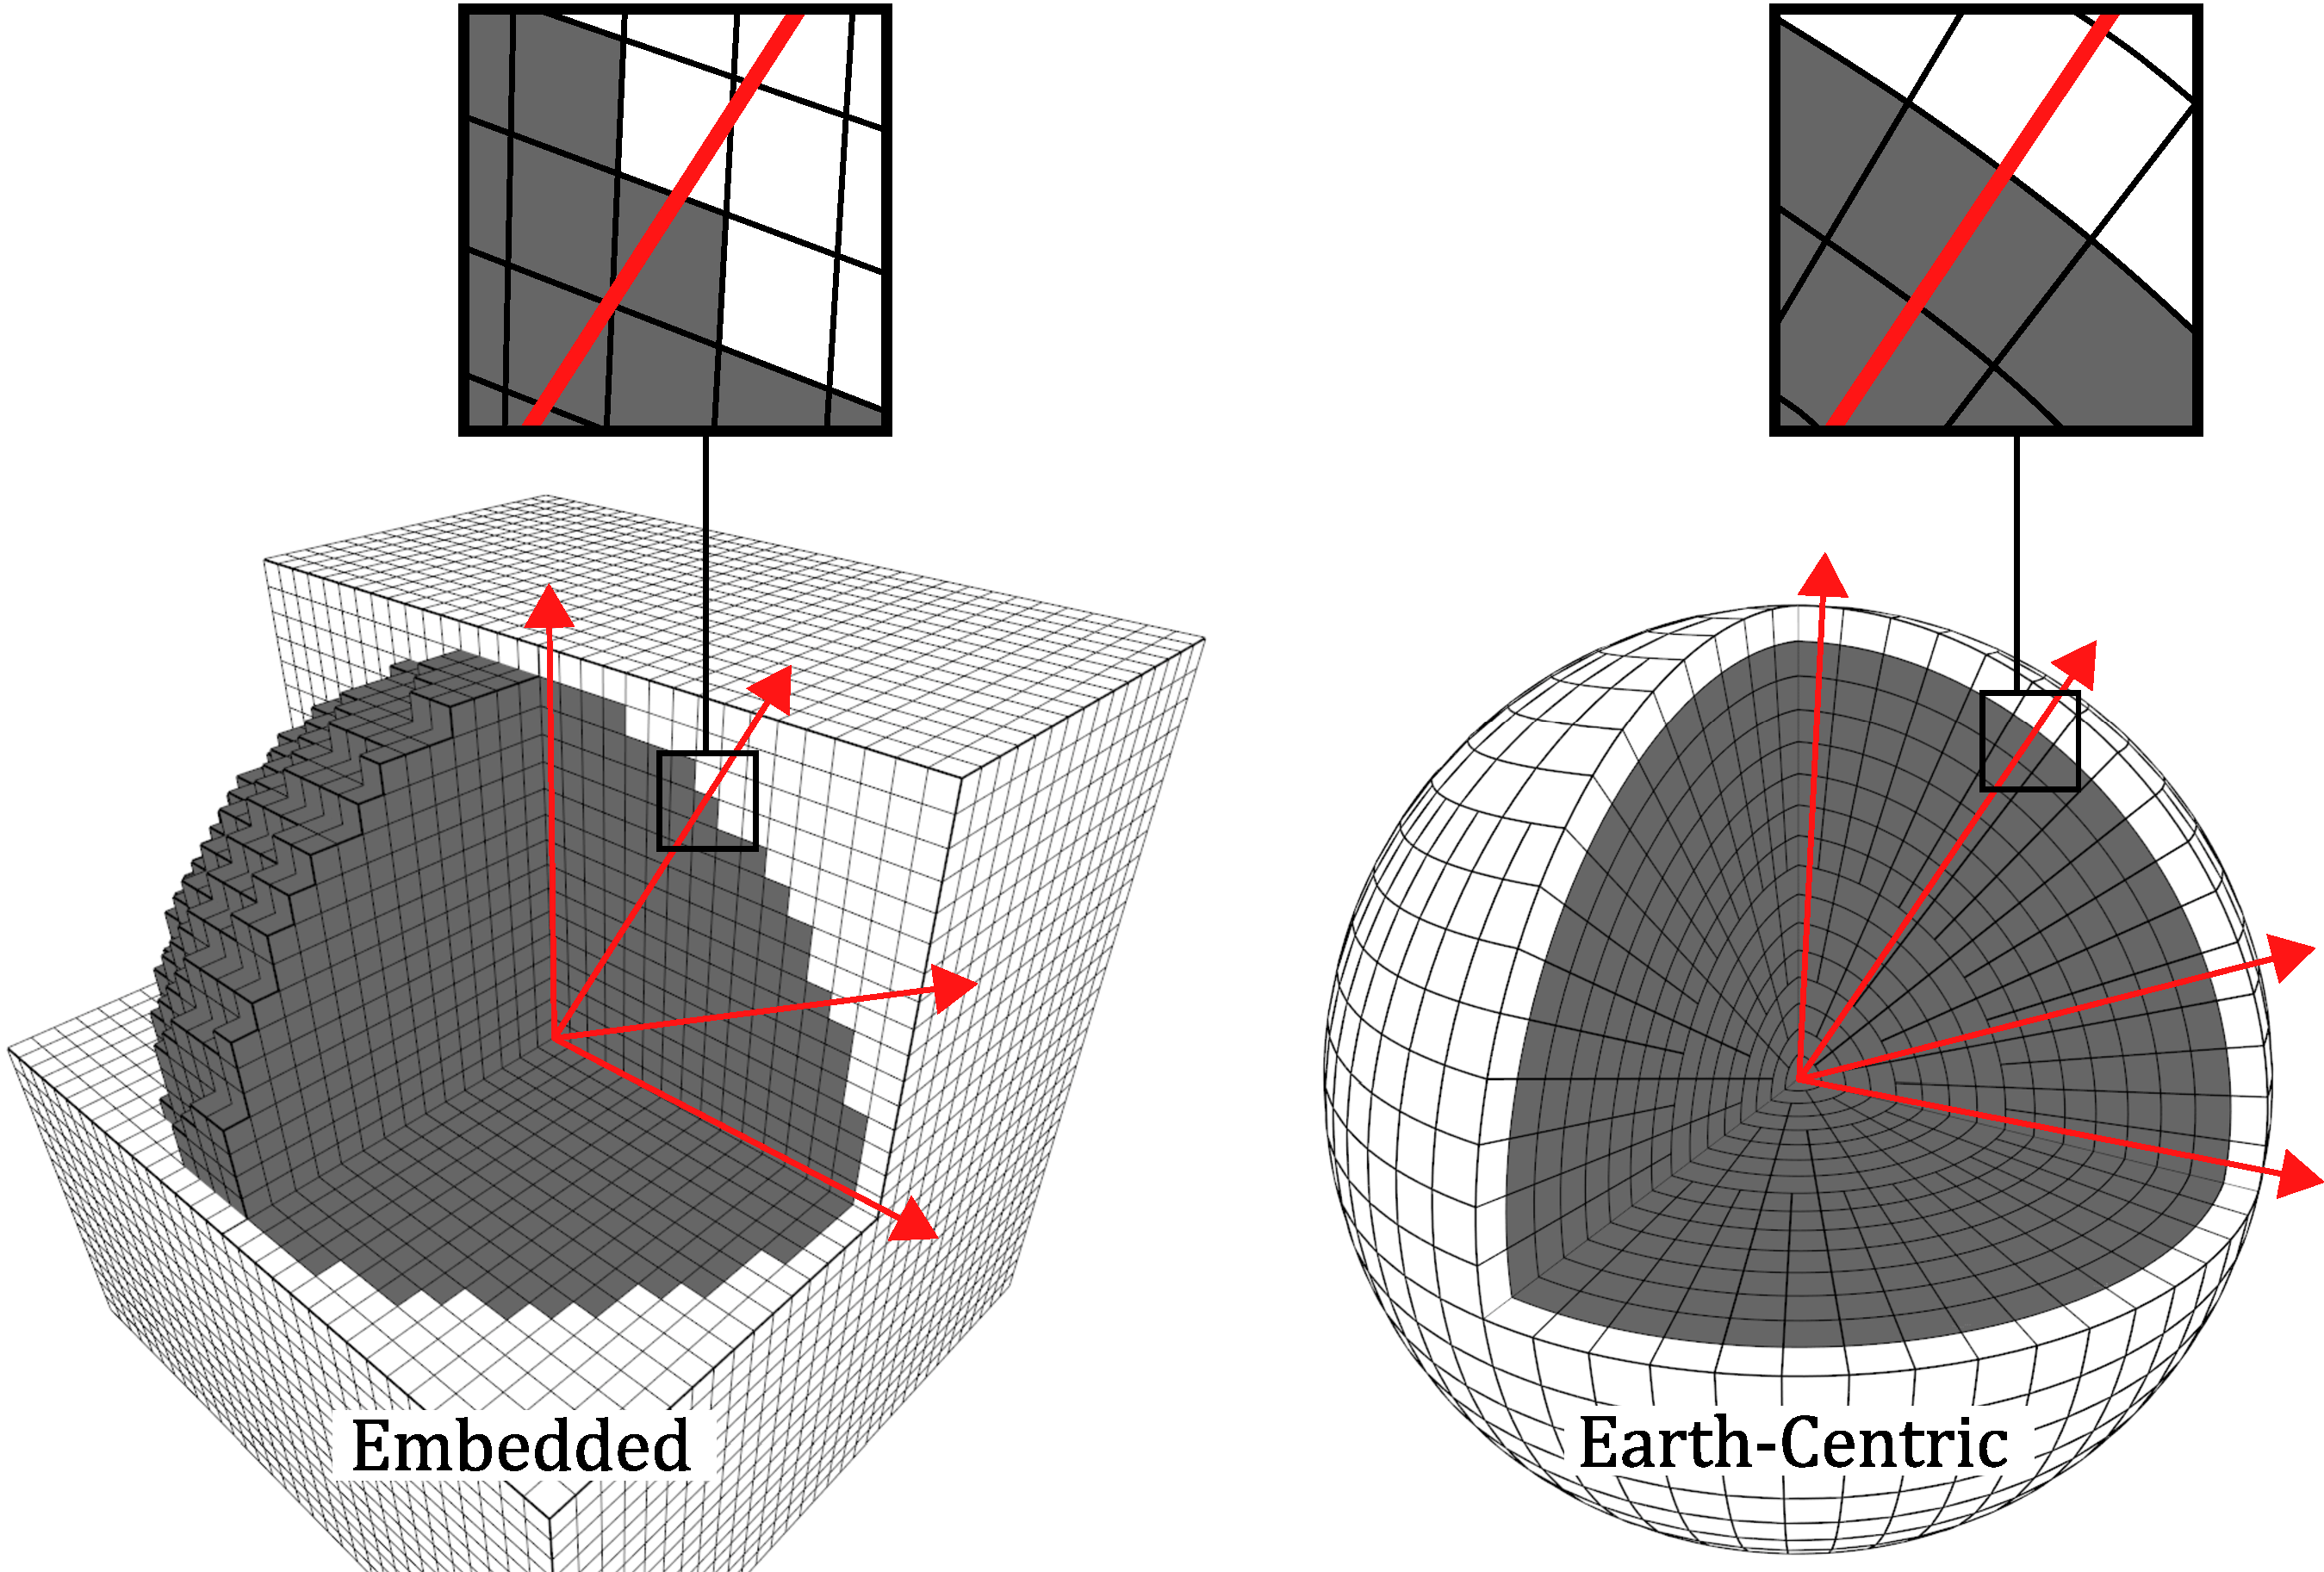
\includegraphics[width=0.85\textwidth]{embed-vs-ec.pdf}
	\caption[Comparison of embedded and Earth-centric approaches for a 3D DGGS]{
		Comparison of a (left) embedded and (right) Earth-centric 3D DGGS.
		Red arrows show directions of increasing altitude.
		Note how with the Earth-centric grid, these arrows are always orthogonal to the upper and lower boundaries of cells.
		This property does not hold in the embedded grid, with arrows intersecting the boundaries of cells at different angles depending on where the cell is located in the grid.
		Image adapted from~\cite{yu2012large-scale}
	}
	\label{fig:embedded}
\end{figure}


Despite the issues present with an embedded grid, for small-scale regions with negligible curvature, these issues also become negligible.
Because of this, embedded grids are frequently used for small-scale objects and phenomena in use cases such as surface building, rock engineering, and reservoir modelling. [citations]
However, the challenges presented by an embedding approach outweigh their benefits in the context of a 3D DGGS, which needs to have global coverage.


The inherent issues with an embedded 3D DGGS stem from the fact that their cells do not align with the Earth's surface and other layers.
Thus far, we have described 3D geospatial data as data with an associated altitude in addition to its surface coordinates, which is a spherical representation of its location.
Therefore, due to the mostly spherical shape of Earth, a 3D DGGS aligned with a sphere (or more accurately, an oblate spheroid) will also be closely aligned with the Earth.
We call this type of 3D DGGS Earth-centric.


\section{Earth-Centric Grids} \label{chap:3:earthCentric}
The most fundamental Earth-centric 3D grid is a direct extension of an LLG to the third dimension (refer back to \cref{fig:3dllg}).
In addition to diving space by latitude and longitude, a 3D LLG also divides space by equal steps in the radial dimension.
Due to the simplicity of its construction, this type of grid has seen use in global crust modelling~\cite{bassin2000current} and exploring P-wave velocity~\cite{zhao2004global}, among other applications.
The GeoSOT3D grid, proposed by Sun and Cheng, is a variation of the standard 3D LLG where latitude and longitude have been extended to larger virtual spaces to improve the efficiency of grid coding~\cite{sun20153d} and has been used to increase the efficiency of aircraft and UAV collision detection~\cite{miao2019low, zhai2019collision}.


Similar radial extensions are also possible for many of the DGG's and DGGS's explored in \cref{chap:2:DGG}.
Being composed of two component LLG's, an extension of the Yin-Yang grid to 3D can be done in the same manner as above.
These 3D Yin-Yang grids have been used extensively for geodynamo and mantle convection simulation~\cite{yoshida2004application, kageyama2005geodynamo, tackley2008modelling}.
Extensions of polyhedron-based DGGS's to 3D have also been done.
An approach by Xie et al. stacks duplicates of a DGGS at increasing radii to create a 3D global grid for interactive volumetric ray tracing of 3D Earth data~\cite{xie2013interactive}.
While this approach is appropriate for the intended use, it is not technically a 3D DGGS, as the radial component of the grid is separate from the cell hierarchy.
In order to incorporate the radial component of the grid with the cell hierarchy, Sirdeshmukh et al. create a 3D (or 4D) DGGS by placing 3D (or 4D) hypercubes on the faces of the DGGS polyhedron~\cite{sirdeshmukh2019utilizing}.
These hypercubes are then refined and traversed with a space-filling curve to create the 3D (or 4D) DGGS, which the authors use to encode point cloud data.


While using a radial extension to create a 3D DGGS is simple and effective, it results in a singularity at the centre of the Earth.
This central singularity causes the same issues near the centre of the grid as seen near the poles of an LLG---namely reduced compactness, a high valence vertex, and an unbounded difference in cell \textit{volume}.
None of the above methods address this central singularity, as these issues are mostly negligible for applications with small ranges of altitudes.
However, in accommodating large altitude ranges (as is the goal of this thesis), these issues become significant and should be addressed.


Similar to how the DQG (\cref{chap:2:spherical}) addresses polar singularities in an LLG, a similar approach can be used for the central singularity in a 3D grid.
A direct extension of the DQG to 3D, known as the spheroid-degenerated octree grid (SDOG), was proposed by Yu and Wu~\cite{yu2009sdog}.
Just as the DQG utilizes a modified quadtree refinement, SDOG extends this refinement to 3D, creating a modified octree refinement.
The resulting cells are relatively uniform in both size and shape, having a bounded maximum difference in volume.
Because of these properties, SDOG has been used for the modelling of large-scale geospatial objects~\cite{yu2012large-scale} and multi-scale visualization of the lithosphere~\cite{yu2012lithosphere}.
We provide a more detailed explanation of SDOG and its specific refinement method in \cref{chap:sdog}.
Another approach similar to SDOG is the Sphere Shell Space 3D Grid, which uses a similarly modified octree refinement of cells but is constructed from multiple spherical shells as opposed to a single sphere~\cite{gang2013sphere}.
Likewise, Wang et al. also apply a similar process to a great circle arc quaternary triangular mesh (QTM) to create a 3D DGGS~\cite{wang2013global}.
These methods all use a similar refinement strategy to handle cell degeneration toward the centre of the grid; however, the terminology used to describe this type of refinement is inconsistent between works.
In this thesis, we propose the term \textit{semiregular degenerate refinement} to describe this class of methods.

\section{3D DGGS Refinement Strategies} \label{chap:3:refinement}

\subsection{Regular Refinement} \label{chap:3:regular}

\subsection{Semiregular Degenerate Refinement} \label{chap:3:semiregDegen}
A regular grid refinement is one that results in regular connectivity in the output domain, henceforth referred to as a regular grid.
For triangular grids, this means each vertex has a valence of exactly six; for quadrilateral grids, a valence of four; and for hexagonal grids, a valence of three.


\begin{figure}[ht!]
	\centering
	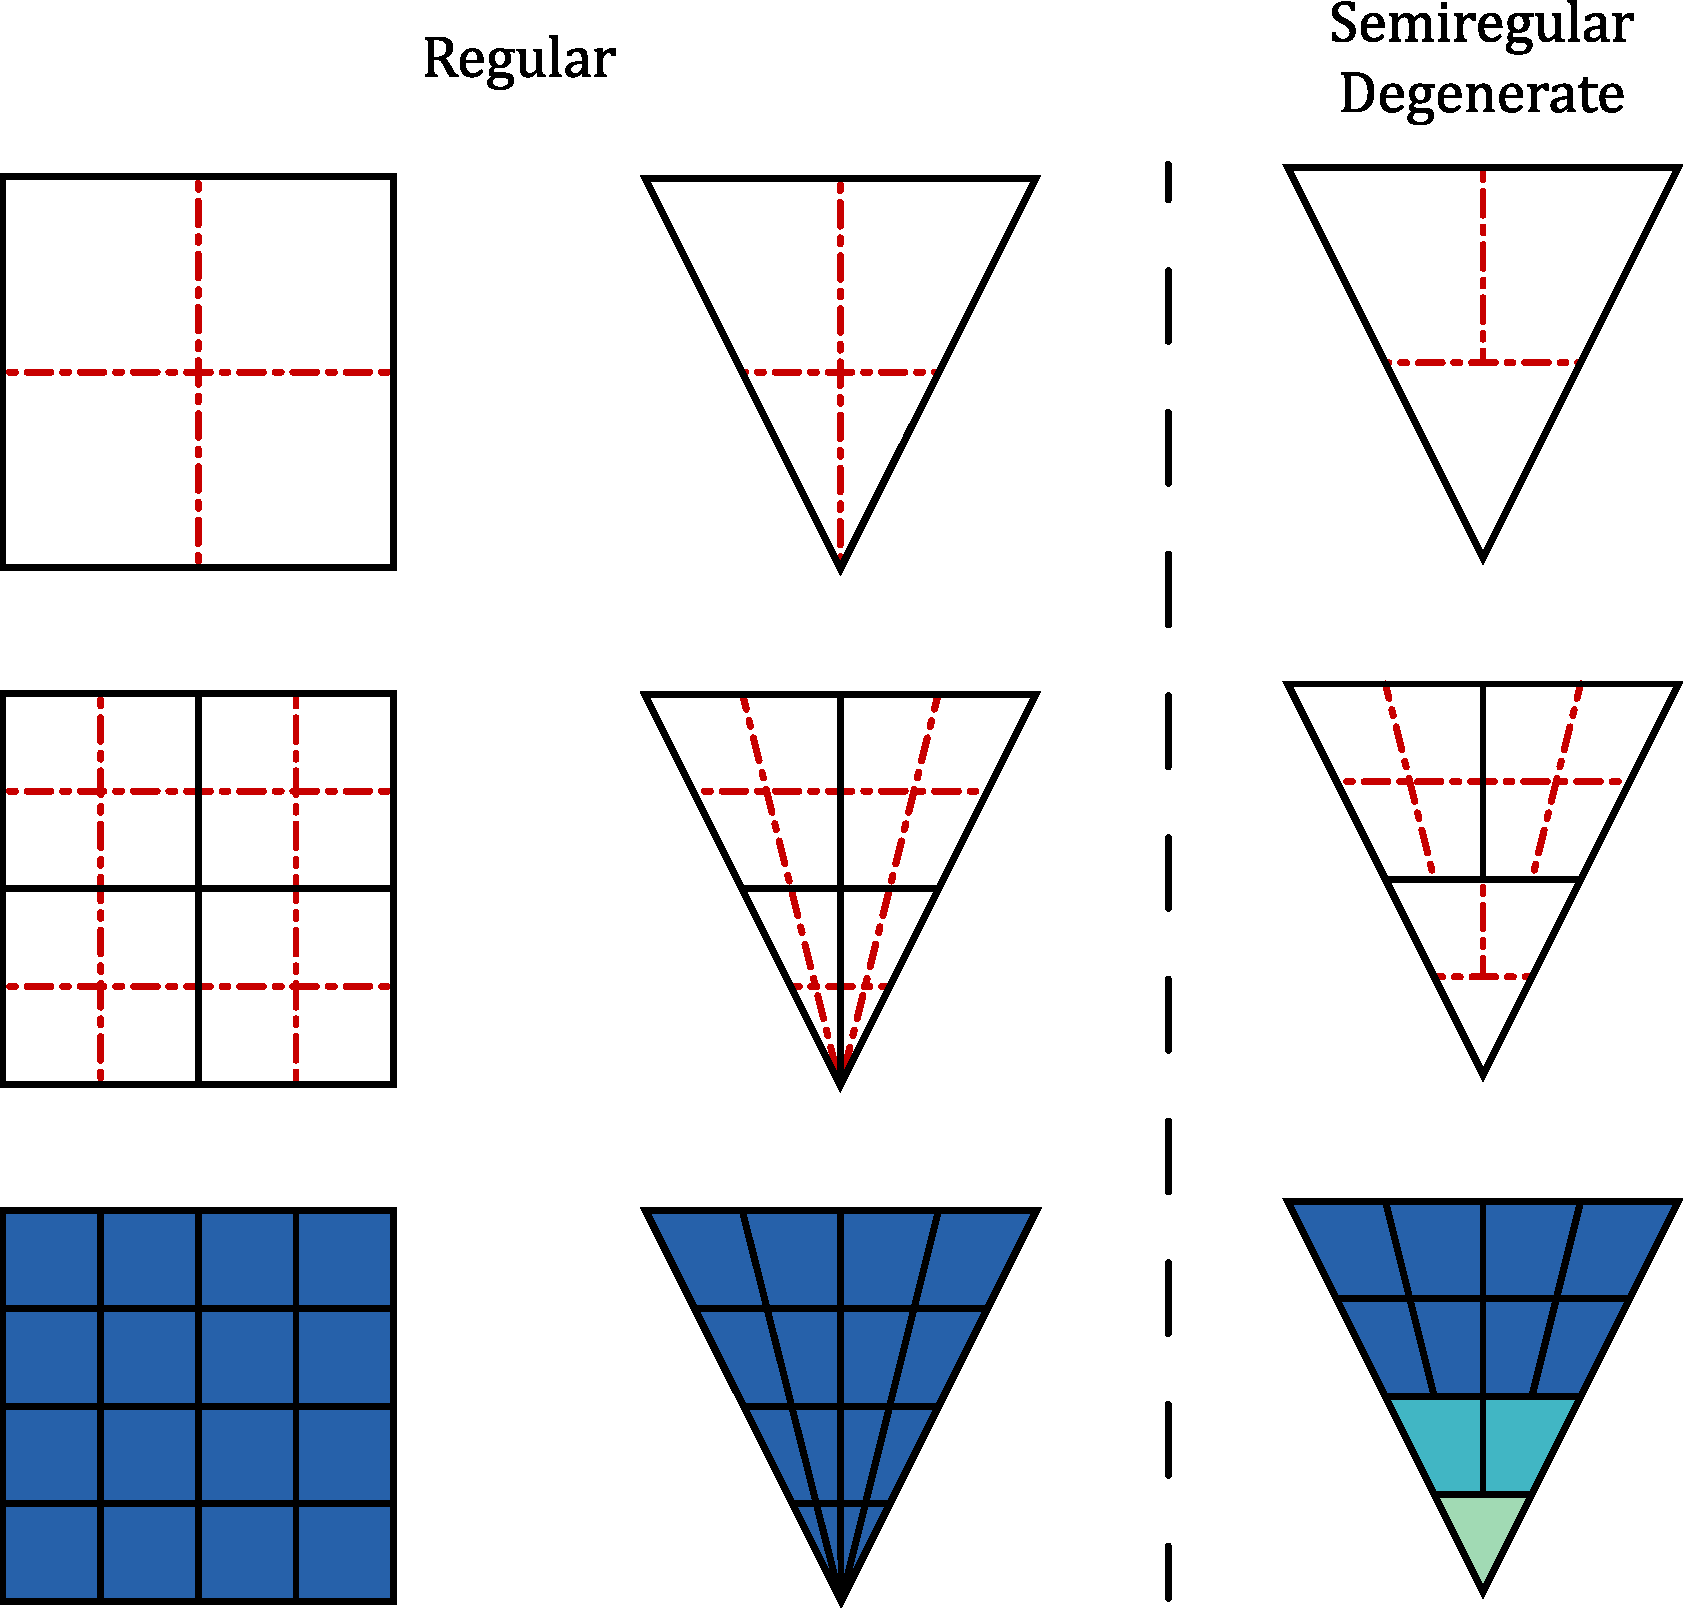
\includegraphics[width=0.7\textwidth]{semireg-degen.pdf}
	\caption[Comparison of regular and semiregular degenerate refinement]{
		A demonstration of regular and semiregular degenerate refinement schemes for quadrilaterals.
		Left: regular refinement applied to a quadrilateral domain.
		Centre: regular refinement applied to a triangular domain.
		Right: semiregular degenerate refinement applied to a triangular domain.
		The bottom row shows regions of regular connectivity in the resulting grids; note how the semiregular degenerate scheme results in several regular regions, but the grid itself is not fully regular
	}
	\label{fig:semireg-degen}
\end{figure}


Looking specifically at regular quadrilateral refinement, one way to achieve this is by splitting each input cell into four output ones with two intersecting straight lines, as shown in \cref{fig:semireg-degen}~left.
As we have seen, applying such a regular refinement to a degenerate (triangular) starting cell---such as spherical octant or a slice going from the surface of a sphere to the centre---still results in a regular grid, but the compactness and size of cells are affected (\cref{fig:semireg-degen}~centre).
To lessen this effect, the splitting edge that would normally intersect the singularity can be stopped at the other edge, as demonstrated in \cref{fig:semireg-degen}~right.
When applying this scheme recursively, only the degenerate (triangular) cells use the special refinement, and non-degenerate (quadrilateral) cells use regular refinement.
As illustrated in \cref{fig:semireg-degen}~bottom, this refinement method results in a grid with regular regions, but the grid as a whole is not itself regular.
Hence, we call this semiregular degenerate refinement.
The same principles apply in 3D for hexahedral grids; however, there are instead three intersecting \textit{faces} used in refinement.
In general, we define a semiregular degenerate refinement to be one in which one or more splitting geometries (curves in 2D and surfaces in 3D) are stopped by another splitting geometry in the direction toward a singularity where, if not stopped, would otherwise intersect said singularity.
Such a definition describes the methods used in DQG, SDOG, Sphere Shell Space 3D Grid, the great circle arc QTM extension, and those used in \cref{chap:extension} of this thesis.


A semiregular degenerate refinement allows for more uniformly sized and compact cells as compared to a regular refinement applied to the same domain.
The main drawback of this class of refinement is the degenerate connectivity introduced between the different semiregular regions of the grid.
In a non-degenerate grid, each cell will have precisely one neighbour along each edge, or no neighbours if the cell is on a boundary of the grid.
In 3D, the same applies but with faces instead of edges.
Grids resulting from semiregular degenerate refinement violate this property, with some cells having multiple neighbours along an edge/face.
Such degenerate connectivity introduces challenges when propagating values across boundaries of cells and calculating values at vertices, as is needed for finite element methods.
There has been work to address this challenge for conventional octrees~\cite{braun2008douar}, which have a similar issue between regions of the grid at different levels of refinement; similar methods could likely be applied to semiregular degenerate grids as well.
Considering the tradeoffs of this approach, we believe the benefits outweigh the disadvantages in the context of a 3D DGGS.
As such, semiregular degenerate refinement is the primary tool used in the remainder of this thesis to achieve the goals set out in \cref{chap:1:goals}.
